\documentclass{beamer}

\usepackage[utf8]{inputenc} % Language and font encoding
\usepackage[icelandic]{babel}
\usepackage[T1]{fontenc}


\usepackage{tikz}
\usepackage[listings,theorems]{tcolorbox}
\usepackage{booktabs}
\usepackage{minted} %Minted and configuration
\usemintedstyle{default}

\renewcommand{\theFancyVerbLine}{\sffamily \arabic{FancyVerbLine}}
%%%%%%%%%%%
% More math
%%%%%%%%%%%
\newcommand{\Mod}[1]{\ \text{mod}\ #1}

%%%%%%%%%%%%%%%%%%%%%%
% Beamer configuration
%%%%%%%%%%%%%%%%%%%%%%
\setbeamertemplate{navigation symbols}{}
\usecolortheme{dove}
\setbeamercolor{frametitle}{fg=white}

\usebackgroundtemplate%
{%
\vbox to \paperheight{

\includegraphics[width=\paperwidth]{Pics/hi-slide-head-2016}

\vfill
\hspace{0.5cm}
\includegraphics[width=0.3\paperwidth]{Pics/hi-von-logo}
\vspace{0.4cm}
    }%
}

\AtBeginSection[]
{
  \begin{frame}<beamer>
    \frametitle{Yfirlit}
    \tableofcontents[currentsection]
  \end{frame}
}

\setbeamerfont{frametitle}{size=\normalsize}
\addtobeamertemplate{frametitle}{}{\vspace*{0.5cm}}

%%%%%%%%%%%%%%%%%%%%%%%%%
% tcolorbox configuration
%%%%%%%%%%%%%%%%%%%%%%%%%

% Setup from: http://tex.stackexchange.com/a/43329/21638
\tcbset{%
    noparskip,
    colback=gray!10, %background color of the box
    colframe=gray!40, %color of frame and title background
    coltext=black, %color of body text
    coltitle=black, %color of title text 
    fonttitle=\bfseries,
    alerted/.style={coltitle=red, colframe=gray!40},
    example/.style={coltitle=black, colframe=green!20, colback=green!5},
}


%%%%%%%%%%%%%%%%%%%%%%%
% Further configuration
%%%%%%%%%%%%%%%%%%%%%%%
\hypersetup{colorlinks=true,pdfauthor={Eirikur Ernir Thorsteinsson},linkcolor=blue,urlcolor=blue}
\graphicspath{{./Pics/}}

\author{Eiríkur Ernir Þorsteinsson}
\institute{Háskóli Íslands}
\date{Haust 2016}

\title{Tölvunarfræði 1a}
\subtitle{Vika 3, seinni fyrirlestur}

\begin{document}

\begin{frame}
\titlepage
\end{frame}

\section{Inngangur}

\begin{frame}{Í síðasta þætti\ldots}
\begin{itemize}
 \item Reiknirit
 \item Undir húddi forritunarmála
 \begin{itemize}
  \item Æðri forritunarmál og vélarmál
  \item Þýðing og túlkun
 \end{itemize}
 \item Forrit í Matlab
 \begin{itemize}
  \item Skipanaskrár
  \item Notendaskilgreind föll
 \end{itemize}
\end{itemize}
Kaflar: 3.1, 3.2, 3.7
\end{frame}

\begin{frame}{Síðasta fyrirlestraræfing}
\begin{center}
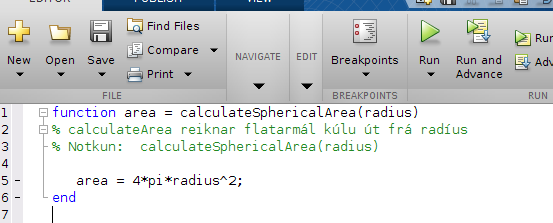
\includegraphics[width=0.9\textwidth]{Pics/spherical-area-function}\\
\vspace{\baselineskip}
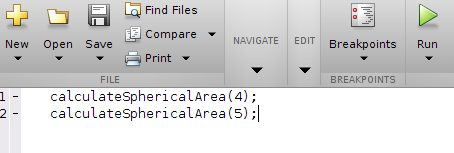
\includegraphics[width=0.9\textwidth]{Pics/spherical-area-script}
\end{center}
\end{frame}

\section{Inntak og úttak (3.3 - 3.4)}

\subsection{Inntak}

\begin{frame}[fragile]{Inntak og úttak}
\begin{itemize}
 \item Skipanaskrárnar í síðasta tíma þurftu að fá gildi inni í skránni
 \begin{itemize}
  \item Til að breyta útreikningum skráarinnar þurfti að breyta skránni
  \begin{itemize}
   \item Ekki mjög sveigjanlegt fyrirkomulag
  \end{itemize}
  \item Föll geta reiknað út úr mismunandi viðföngum, en skipanaskrár þurfa aðrar aðferðir
 \end{itemize}
\end{itemize}
\begin{minted}[frame=lines]{matlab}
% Þessi skrá reiknar flatarmál hrings

radius = 5;
area = pi * (radius^2);
\end{minted}
\end{frame}

\begin{frame}[fragile]{Inntaksfallið input}
\begin{itemize}
 \item Matlab hefur inntaksfallið \texttt{input}
 \begin{itemize}
  \item Hættir keyrslu skipana (ef í skipanaskrá), birtir skilaboð og bíður eftir inntaki notanda
  \item Haldið er áfram eftir að notandinn hefur smellt á Enter/Return
 \end{itemize}
\end{itemize}

\begin{minted}[frame=lines]{matlab}
>> radius = input('Sláið inn radíus: ')
Sláið inn radíus: 5
radius =
     5
\end{minted}
\end{frame}

\begin{frame}[fragile]{Inntaksfallið input}
\begin{itemize}
 \item Fallið \texttt{input} býst við að fá tölu frá notanda
 \begin{itemize}
  \item Ef inntakið á að vera texti, þá þarf að taka það fram
  \item Eyður koma með ef það eru aðrir stafir með, annars er breytan tóm
 \end{itemize}
\end{itemize}

\begin{minted}[frame=lines]{matlab}
>> name = input('Nafn notanda: ', 's')
Nafn notanda: Eiríkur Ernir
name = 
      Eiríkur Ernir
\end{minted}
\end{frame}

\begin{frame}{Input í forritum}
\begin{itemize}
 \item \texttt{input} er venjulega notað í skipanaskrám
 \begin{itemize}
  \item Þá er oftast sett semíkomma á eftir input-skipuninni til að notandinn sé ekki truflaður
 \end{itemize}
 \item \texttt{input} er venjulega \textbf{ekki} notað í föllum
 \item \ldots nema fallið hafi það sérstaka hlutverk að taka við inntaki
 \begin{itemize}
  \item Í föllum er venjulega talið æskilegt að gildi niðurstöðunnar velti að sem mestu leyti á inntaksstikum og helst engu öðru
 \end{itemize}
\end{itemize}
\end{frame}

\begin{frame}{3 skref í lausnaraðferð}
\begin{enumerate}
 \item Fá inntak
 \begin{itemize}
  \item Lesa af lyklaborði frá notenda, lesa úr skrá, 
 \end{itemize}
 \item Framkvæma útreikninga
 \begin{itemize}
  \item Tekur mislangan tíma
 \end{itemize}
 \item Birta niðurstöðu
 \begin{itemize}
  \item Skrifa í skrá, birta á skjá
  \item Gera niðurstöðu skiljanlega
 \end{itemize}
\end{enumerate}
\end{frame}

\subsection{Úttak}

\begin{frame}[fragile]{Úttaksföll}
\begin{itemize}
 \item Matlab hefur tvö föll til að sýna úttak
 \begin{itemize}
  \item \texttt{disp}: Skrifar út gildi inntaksins
  \item \texttt{fprintf}: Skrifar út gildi á ákveðnu sniði
 \end{itemize}
\end{itemize}
\begin{minted}[frame=single]{matlab}
>> disp(2^10)
 1024
>> fprintf('Flatarmálið er %d metrar\n',5*4)
Flatarmálið er 20 metrar
\end{minted}
\end{frame}

\begin{frame}{disp fallið}
\begin{itemize}
 \item Einfalt fall til að birta niðurstöður reikninga
 \begin{itemize}
  \item Svipað og þegar vantar semíkommu í skipanaglugga
  \begin{itemize}
   \item Oft örlítið snyrtilegra, samt
  \end{itemize}
  \item Getur verið erfitt að blanda saman texta og tölum í úttakinu
  \item Notað ef ekki eru miklar kröfur um flott úttak
 \end{itemize}
\end{itemize}
\end{frame}

\begin{frame}{fprintf fallið}
\begin{itemize}
 \item Notar sniðstreng (e. \emph{format string}) til að stýra útliti úttaks
 \item Kemur úr forritunarmálinu C
 \begin{itemize}
  \item Stendur fyrir \textbf{F}ile \textbf{Print} \textbf{F}ormatted
  \item Ekki talið sérstaklega elegant fram sett, en virkar vel
 \end{itemize}
 \item Almennt form:
 \begin{itemize}
  \item \texttt{fprintf('snið', a1, a2, \ldots )}
 \end{itemize}
 \item 'Snið' lýsir því hvernig gildin a1, a2, ... eru birt
 \begin{itemize}
  \item Getur innihaldið ýmislegt - t.d. texta og ``lausnarstafi''
 \end{itemize}

\end{itemize}
\end{frame}

\begin{frame}[fragile]{Dæmi um notkun fprintf}
Skipanaskrá sem framkvæmir fjölda útreikninga gæti viljað prenta út gildin svo að þau raðist fallega upp.

\begin{minted}[frame=lines]{matlab}
>> fprintf('Keyrsla %d: f(x)=%5.2f\n', i, fx)
Keyrsla 6: f(x)= 0.14
\end{minted}

(Gerir ráð fyrir \texttt{i = 6} og \texttt{fx = 0.14}.)

\end{frame}

\begin{frame}{Sniðslýsingar}
\begin{columns}
\column{0.5\textwidth}
\begin{itemize}
 \item Segja til um hvernig gildin sem koma á eftir eiga að birtast
 \begin{itemize}
  \item Byrjar á \%
  \item Svo kemur heildarbreidd sviðsins (tala)
  \item Síðan getur komið fjöldi aukastafa
  \item Sniðstegund
 \end{itemize}
\end{itemize}
\column{0.5\textwidth}
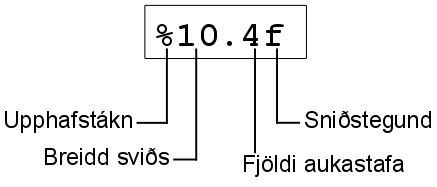
\includegraphics[width=\linewidth]{Pics/format}
\end{columns}
\end{frame}

\begin{frame}{Sniðstegundir í fprintf}
\begin{center}
\begin{tabular}{ll}
\toprule
Sniðstegund&Merking\\
\midrule
\%$n$\texttt{d} &Heiltala í $n$ stafa svæði\\
\%$n$.$m$\texttt{f}&Kommutala í $n$ stafa svæði með $m$ aukastöfum\footnote{ath. að $n$ er heildarstærðin}\\
\%$n$.$m$\texttt{e}&Kommutala á veldisformi (t.d. \texttt{3.141e+00})\\
\%$n$\texttt{s}&Strengur í $n$ stafa svæði\\
\bottomrule
\end{tabular}
\end{center}
Ef breidd sviðs vantar þá er sviðið gert nógu stórt fyrir gildið sem á að sýna
\end{frame}

\begin{frame}{Lausnarstafir í fprintf}
Lausnarstafir (e. \emph{escape characters}) eru notaðir til að sýna ýmislegt sem ekki er texti eða tölur.
\begin{center}
\begin{tabular}{ll}
\toprule
Sniðstegund&\\
\midrule
\texttt{\textbackslash{}n}&Ný lína\\
\texttt{\textbackslash{}t}&``tab'' (þ.e. dálkstaðsetning)\\
\texttt{''}&Táknið \texttt{'}\\
\texttt{\%\%}&Táknið \%\\
\texttt{\textbackslash\textbackslash}&Táknið \textbackslash\\
\bottomrule
\end{tabular}
\end{center}
\end{frame}

\begin{frame}[fragile]{Vigrar og fylki í fprintf}
Skoðun kennarans: Vigrar og fylki eru erfið meðförum í \texttt{fprintf}.
\vspace{\baselineskip}
\begin{columns}
\column{0.6\textwidth}
Fylki eru prentuð út með línulegri röðun - dálk fyrir dálk
\begin{minted}[frame=lines]{matlab}
>> a = randi(5,2,2); % 2x2 fylki
>> fprintf('Fylkið er %d\n', a)
Fylkið er 4
Fylkið er 1
Fylkið er 4
Fylkið er 5
\end{minted}
\column{0.4\textwidth}
Bendill endar í vitlausri línu
\begin{minted}[frame=lines]{matlab}
>> v = 2:6;
>> fprintf('%3d', v)
  2  3  4  5  6>>
\end{minted}
\end{columns}

\end{frame}


\begin{frame}{Fyrirlestraræfing}
Skráið ykkur inn á \url{http://socrative.com/} og gerið fyrstu tvær spurningarnar

Herbergisnúmer = \texttt{TOL105G2016}

Notendanafn = HÍ-tölvupóstfang
\end{frame}

\section{Einfaldar myndir (3.5)}

\begin{frame}{Einfaldar myndir í Matlab}
\begin{itemize}
 \item Matlab hefur fjölmargar leiðir til að sýna gögn á myndrænan hátt.
 \begin{itemize}
  \item Línurit
  \item Súlurit
  \item Kökurit
  \item Punktarit
  \item Hæðarlitir
  \item Einnig til þrívíðar útgáfur
 \end{itemize}
\end{itemize}
\end{frame}

\begin{frame}{Dæmi um mynd úr Matlab}
\vspace{2\baselineskip}
\begin{center}
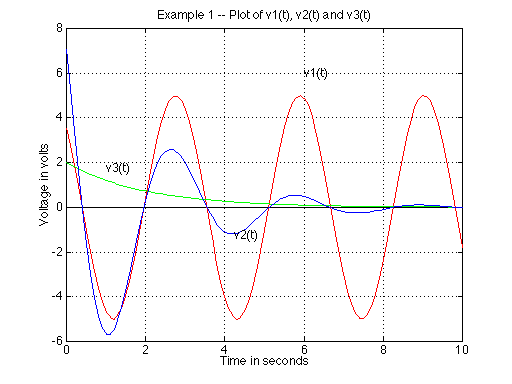
\includegraphics[height=0.6\textheight]{Pics/plot-example1}
\end{center}\footnote{Þessi mynd, sem og aðrar í seríunni, eru fundnar á Google.}
\end{frame}

\begin{frame}{Dæmi um mynd úr Matlab}
\begin{center}
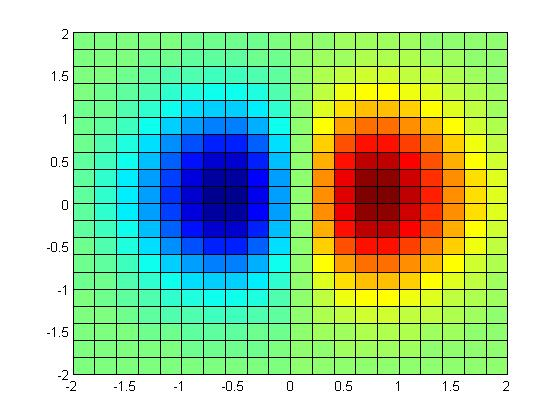
\includegraphics[width=0.8\textwidth]{Pics/plot-example2}
\end{center}
\end{frame}

\begin{frame}{Dæmi um mynd úr Matlab}
\begin{center}
\vspace{\baselineskip}
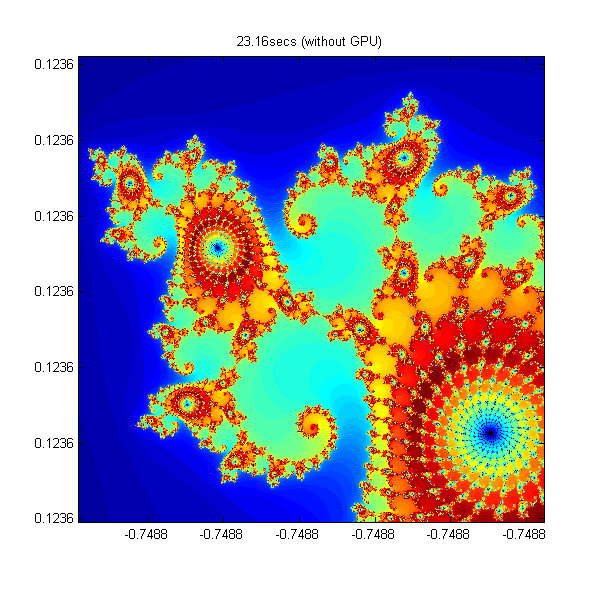
\includegraphics[width=0.6\textwidth]{Pics/plot-example3}
\end{center}
\end{frame}

\begin{frame}{Dæmi um mynd úr Matlab}
\begin{center}
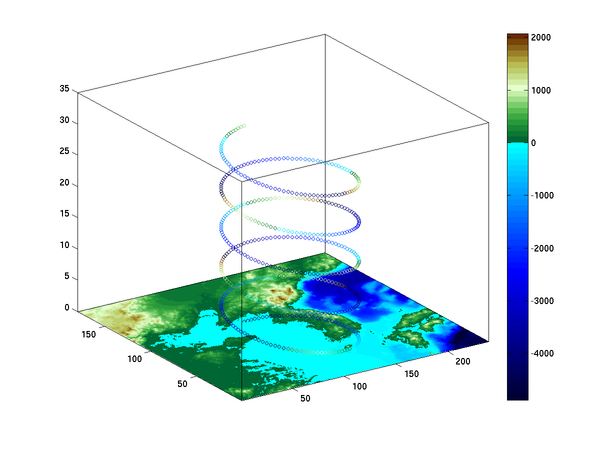
\includegraphics[width=0.8\textwidth]{Pics/plot-example4}
\end{center}
\end{frame}

\begin{frame}[fragile]{Teiknifallið plot}
\vspace{\baselineskip}
\begin{columns}
\column{0.5\textwidth}
\begin{itemize}
 \item Mest notaða teiknifallið er \texttt{plot}
 \begin{itemize}
  \item Tekur inn vigra fyrir $x$ og $y$ og teiknar línurit
  \item Ásarnir eru kvarðaðir sjálfkrafa
 \end{itemize}
\end{itemize}
\begin{minted}[frame=lines]{matlab}
>> x = 1:6;
>> y = randi([0, 10],1,6);
>> plot(x,y)
\end{minted}

\column{0.5\textwidth}
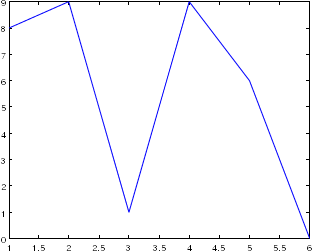
\includegraphics[width=\linewidth]{Pics/plot-example5}
\end{columns}
\end{frame}

\begin{frame}{Ýmsar stillingar á plot}
\vspace{\baselineskip}
\begin{columns}
\column{0.6\textwidth}
\begin{itemize}
 \item Hægt er að setja kvarða á ásana:
 \begin{itemize}
  \item \texttt{>> axis([1, 6, 0, 12])}
  \item Sniðið er \texttt{[xmin, xmax, ymin, ymax]}
 \end{itemize}
 \item Setja má merki á ásana:
 \begin{itemize}
  \item \texttt{>> xlabel('Nemandi')}
  \item \texttt{>> ylabel('Einkunn')}
 \end{itemize}
 \item Titill á línuritið:
 \begin{itemize}
  \item \texttt{>> title('Nemendur og einkunnir')}
 \end{itemize}
\end{itemize}

\column{0.4\textwidth}
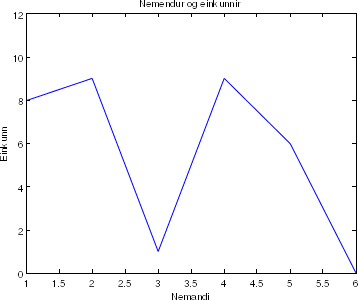
\includegraphics[width=\linewidth]{Pics/plot-example6}
\end{columns}
\end{frame}

\begin{frame}{Stillingar línurits}
\vspace{2\baselineskip}
3. viðfangið í plot fallinu eru stafir sem lýsir gerð línuritsins.\footnote{Sjálfgefin stilling er \texttt{plot(x, y, 'b -')}}\\
\texttt{>> plot(x, y, '}\emph{lmt}\texttt{')} $\leftarrow$ \textbf{l}itur, \textbf{m}erki, \textbf{t}egund.\\
\vspace{0.5\baselineskip}
\begin{columns}
\small
\column{0.33\textwidth}
\begin{tabular}{cl}
\toprule
Merki&Litur\\
\midrule
\texttt{b}&blár\\
\texttt{g}&grænn\\
\texttt{r}&rauður\\
\texttt{c}&blágrænn\\
\texttt{m}&blárauður\\
\texttt{y}&gulur\\
\texttt{k}&svartur\\
\bottomrule
\end{tabular}
\column{0.33\textwidth}
\begin{tabular}{cl}
\toprule
Merki&Útkoma\\
\midrule
\texttt{.}&punktur\\
\texttt{o}&hringur\\
\texttt{x}&x-tákn\\
\texttt{+}&plús-tákn\\
\texttt{*}&stjarna\\
\texttt{s}&ferningur\\
\texttt{d}&tígull\\
\texttt{v}&þríhyrningur\\
\texttt{\^{}}&þríhyrningur\\
\bottomrule
\end{tabular}
\column{0.33\textwidth}
\begin{tabular}{cl}
\toprule
Merki&Tegund\\
\midrule
\texttt{-}&heil lína\\
\texttt{:}&punktalína\\
\texttt{-.}&strik-punktur\\
\texttt{--}&strikalína\\
\texttt{ }&engin lína\\
\bottomrule
\end{tabular}
\end{columns}
\end{frame}

\begin{frame}[fragile]{Dæmi um línurit}

\begin{columns}
\column{0.5\textwidth}
\begin{minted}[frame=lines]{matlab}
>> plot(x, y, 'r*')
\end{minted}
Rautt, stjörnur og engin lína
\column{0.5\textwidth}
\begin{center}
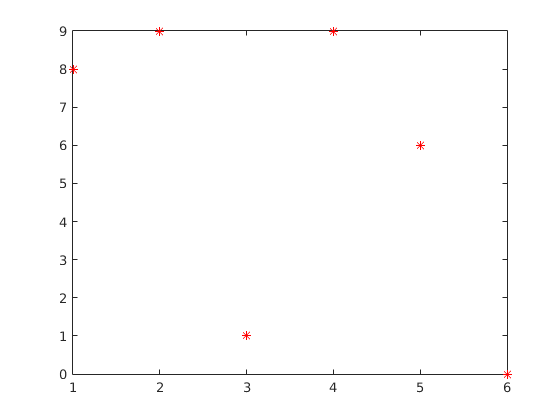
\includegraphics[width=0.7\linewidth]{Pics/plot-example7}
\end{center}
\end{columns}
\vspace{\baselineskip}
\begin{columns}
\column{0.5\textwidth}
\begin{minted}[frame=lines]{matlab}
plot(x, y, 'bo:')
\end{minted}
Blátt, hringir og punktalína
\column{0.5\textwidth}
\begin{center}
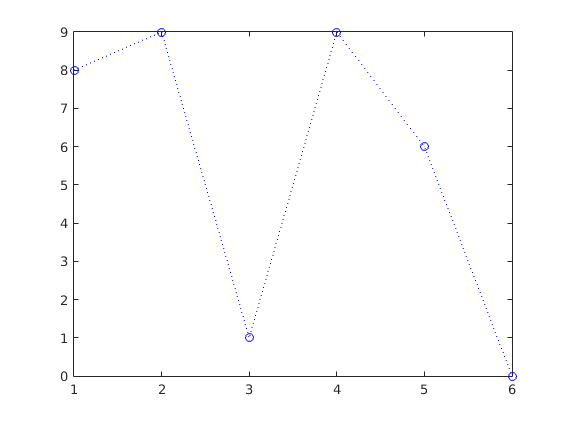
\includegraphics[width=0.7\linewidth]{Pics/plot-example8}
\end{center}
\end{columns}
\end{frame}

\begin{frame}{Nokkrar skipanir fyrir línurit}
\begin{center}
\begin{tabular}{lp{8cm}}
\toprule
Skipun&Áhrif\\
\midrule
\texttt{clf}&Hreinsar myndaglugga (fyrir endurteiknun)\\
\texttt{close}&Lokar opnum glugga\\
\texttt{figure}&Opnar nýjan tóman myndaglugga (fyrir margar aðskildar myndir)\\
\texttt{hold on}&Festir myndaglugga (fyrir margar myndir hver ofan á annarri)\\
\texttt{legend}&Merkir línuritið með útskýringartexta\\
\texttt{grid}&Setur rúðustrikun á myndagluggann\\
\bottomrule
\end{tabular}
\end{center}

\end{frame}

\begin{frame}{Ráðleggingar fyrir teikningu}
\begin{itemize}
 \item Notið skipanaskrár til að halda utan um teikningar
 \begin{itemize}
  \item Ef um afmarkaða, endurnýtanlega útreikninga er að ræða, framkvæmið þá í sérstöku falli (önnur skrá)
 \end{itemize}
 \item Auðvelt er að teikna á vitlausan glugga eða utan hans
 \begin{itemize}
  \item Verið meðvituð um núverandi stöðu forritsins
  \item \texttt{clear} og \texttt{close} geta komið að góðum notum
 \end{itemize}
 \item Eins og alltaf eru \texttt{help} og \texttt{doc} vinir ykkar!
\end{itemize}
\end{frame}

\section{Einföld skráarnotkun (3.6)}

\begin{frame}{Einfalt inntak og útták með skrám}
\begin{itemize}
 \item Þegar unnið er með mikið gagnamagn er gott að geyma gögn í skrám
 \item Skipunin \texttt{save skráarnafn fylki -ascii} vistar gögnin í $fylki$ í skrá
 \begin{itemize}
  \item Ef skráin er þegar til er hún yfirskrifuð
  \item Skrifa má aftast í skrá í stað yfirskriftar með því að gefa valmöguleikann \texttt{-append}
 \end{itemize}
 \item Skipunin \texttt{load skráarnafn} les innihald skrár inní fylki
  \begin{itemize}
   \item Fylkið heitir sama nafni og skráin (án endingar)
  \end{itemize}
 \end{itemize}
\end{frame}

\begin{frame}[fragile]{Dæmi um skráarinntak og skráarúttak}
\begin{minted}[frame=lines]{matlab}
>> a = randi(5,2,2) % 2x2 slembifylki búið til
a =
   3   2
   3   4
>> save gogn.dat a -ascii % a skrifað í skrána gogn.dat
>> load gogn.dat % innihald gogn.dat sett í breytuna gogn
>> gogn
gogn =
   3   2
   3   4
\end{minted}
\end{frame}

\begin{frame}{Fyrirlestraræfing}
\begin{columns}
\column{0.7\textwidth}
Skráið ykkur inn á \url{http://socrative.com/} og klárið æfinguna.

Herbergisnúmer = \texttt{TOL105G2016}

Notendanafn = HÍ-tölvupóstfang
\column{0.3\textwidth}
\begin{center}
\begin{tabular}{ll}
\toprule
Klst&$C^\circ$\\
\midrule
0&12.5\\
3&12.4\\
6&12.3\\
9&12.8\\
12&13.4\\
15&14\\
18&13.1\\
21&12.8\\
\bottomrule
\end{tabular}
\end{center}
\end{columns}

\end{frame}



\end{document}
